%!TEX root = ../dissertation.tex
\begin{savequote}[75mm]
Most people stop looking when they find the proverbial needle in the haystack. I would continue looking to see if there were other needles.
\qauthor{-Albert Einstein}
\end{savequote}

\chapter{Identification of genetic outliers due to sub-structure and cryptic relationships}

\newthought{In order to minimize} the effects of genetic confounding on the analysis of high-throughput genetic association studies, e.g. (whole-genome) sequencing (WGS) studies, genome-wide association studies (GWAS), etc., we propose a general framework to assess and to test formally for genetic heterogeneity among study subjects. As the approach fully utilizes the recent ancestor information captured by rare variants, it is especially powerful in WGS studies. Even for relatively moderate sample sizes, the proposed testing framework is able to identify study subjects that are genetically too similar, e.g cryptic relationships, or that are genetically too different, e.g. population substructure. The approach is computationally fast, enabling the application to whole-genome sequencing data, and straightforward to implement.\\
 \textbf{Results:} Simulation studies illustrate the overall performance of our approach. In an application to the 1000 Genomes Project, we outline an analysis/cleaning pipeline that utilizes our approach to formally assess whether study subjects are related and whether population substructure is present. In the analysis of the 1000 Genomes Project data, our approach revealed subjects that are most likely related, but had previously passed standard qc-filters. \\
\textbf{Availability:} An implementation of our method, Similarity Test for Estimating Genetic Outliers (STEGO), is available in the R package stego from Github at \\ https://github.com/dschlauch/stego.


\section{Introduction}

The fundamental assumption in standard genetic association analysis
is that the study subjects are independent and that, at each locus,
the allele frequency is identical across study subjects (\citealp{choi2009case,purcell2007plink,yang2010common}).
In the presence of population heterogeneity, e.g. population substructure
or cryptic relatedness, these assumptions are violated. It can introduce
confounding into the analysis and lead to biased results, e.g. false
positive findings (\citealp{price2006principal,kang2010variance,ptak2002evidence,voight2005confounding}).
Given the generality of the problem, it has been the focus of methodology
research for a long time. An early approach, genomic control, was developed for candidate gene and later for genome-wide association studies (GWAS)  (\citealp{devlin2001genomic,bacanu2002association}), adjusting the association test statistics at the loci of
interest by an inflation factor that is estimated at a set of known
null-loci. With the arrival of GWAS data, it became possible to estimate
the genetic dependence between study subjects and the overall genetic
variation for each study subject by computing the empirical genetic
variance-covariance matrix between study subjects at a whole genome
level. The genetic variance-covariance matrix can then be utilized
in two ways to minimize the effects of population substructure on
the association analysis. 

The first method is to compute an eigendecomposition of the matrix
and to include the eigenvectors that explain the most variation as
covariates in the association analysis (\citealp{price2006principal,price2010new}).
An alternative approach is to incorporate the estimated dependence
structure of the study subjects directly into a generalized linear
model and account directly for the dependence at the model-level (\citealp{listgarten2012improved,lippert2011fast,zhang2010mixed}).
Both approaches have proven to work well in numerous applications.
While the first approach is computationally fast and easy to implement,
the direct modeling of the dependence structure between study subjects
can be more efficient (\citealp{mathieson2012differential}). 

However, both approaches benefit if, prior to the analysis, study
subjects whose genetic profile is very different from the other study
subjects, e.g. ``genetic outliers'',
are removed from the data set. A common practice is currently
to examine the eigenvalue plots visually and to identify outliers
by personal judgment on how far study subjects are from the ``clouds''
of study subjects. As typically up to 10 eigenvectors have to be considered,
this process of identifying outliers can become a complicated and
subjective procedure. Alternatively, a software tool SMARTPCA (\citealp{patterson2006population}), provides a more quantitative utility for removal of outliers by iteratively recomputing PCs in the genetic data.  The method assumes a set of unrelated individuals and uses the covariance-based genetic similarity matrix to identify these individuals.

Many methods exist for inferring relatedness which make the strong
assumption of population homogeneity (\citealp{purcell2007plink,yang2010common,kang2010variance,choi2009case}).
These methods have been shown to be biased in the context of population
heterogeneity (\citealp{manichaikul2010robust}). More recently, methods
have been developed which attempt to estimate relatedness
with population structure (\citealp{thornton2012estimating,manichaikul2010robust}).
These developments improve the ability to detect existing pedigrees,
which can aid in the removal of individuals who violate homogeneity.
However, there is currently no quantitative measure of homogeneity
which can be used to test a dataset prior to the application of GWAS.

In this communication, we propose a formal statistical test that assesses
whether two study subjects come from the same population and whether
they are unrelated. The test statistic is based on an adaptation of
the Jaccard Index which utilizes the idea that variants are differentially
informative of relatedness based on their allele frequency. Recent
work has shown that the Jaccard Index alone can be used to reveal
finer scale population structure compared with existing methods such
as EIGENSTRAT (\citealp{prokopenko2016utilizing}). Furthermore, the distribution
of our statistic can be derived under the null-hypothesis which makes
it computationally fast, enabling the application to whole-genome
sequencing data. Our measure has clearly defined properties which
can be used to test for homogeneity in a population and in particular
identify individuals who are likely be related in a study population.
Applications to the 1,000 Genome Project suggests that our approach
is better suited to detect sub-populations than genetic variance-covariance
approach. This is most likely attributable to the emphasis of our
approach on small allele frequencies.


\section{Methods}

Exploiting the information in rare variants (RVs), such as one with
minor allele frequency (MAF) < 1\%, is fundamental to our method,
as our approach utilizes the features of RVs that they are typically
more recent than common variants and that many of them are population/family
specific. Since allele frequencies can differentially confound association
studies (\citealp{mathieson2012differential}), we developed a method that
utilizes the differential informativeness of variants by allele frequency
to obtain a high resolution picture of population structure and protect
the association study against bias due to genetic confounding. Our
approach uses an intuitive, computationally straightforward approach
towards identifying similarity between two study subjects which is
also directly linked to the kinship coefficient. 

\subsection{Similarity measure among haploid genomes}

Consider a matrix of $n$ individuals ($2n$ haploid genomes), with
$N$ independent variants described by the genotype matrix $\mathbf{G}_{2n\times N}$.
$\mathbf{G}$ is a binary matrix with value $1$ indicating the presence
of the minor allele and $0$ indicating the major allele. We define
the similarity index between two haploid genomes, $s_{i,j}$

\begin{equation}
s_{i,j}=\frac{\sum_{k=1}^{N}w_{k}\mathbf{G}_{i,k}\mathbf{G}_{j,k}}{\sum_{k=1}^{N}I\left[\sum_{l=1}^{2n}\mathbf{G}_{l,k}>1\right]}\label{eq:s equation}
\end{equation}

where 

\[
w_{k}=\begin{cases}
\frac{{2n \choose 2}}{{\sum_{l=1}^{2n}\mathbf{G}_{l,k} \choose 2}} & \text{if } \sum_{l=1}^{2n}\mathbf{G}_{l,k}>1\\
0 & \text{if } \sum_{l=1}^{2n}\mathbf{G}_{l,k}\le1
\end{cases}
\]

and $I[\cdot]$ is an indicator function, evaluating to $1$ if true and $0$ if false.

We can consider the weight variable, $w_k$, to be the inverse of the probability that two alleles selected randomly without replacement both belong to the set of minor alleles.  Intuitively, for $\sum_{l=1}^{2n}\mathbf{G}_{l,k}>1$, $w_k$ is monotonically decreasing as the minor allele count increases (See below).

In the absence of population structure, i.e. homogeneous population
we have
\begin{equation}
E\left(s_{i,j}\right)=1
\label{eq:expectation_equation}
\end{equation}

It therefore follows from the Central Limit Theorem that in the absence
of population structure, cryptic relatedness and dependence between
loci (such as linkage disequilibrium) the distribution of the similarity
index, $s_{i,j}$ is Gaussian.
\[
s_{i,j}\sim N\left(1,\sigma_{i,j}^{2}\right)
\]
Where the variance of $s_{ij}$ can be estimated by 
\begin{equation}
\hat{\sigma_{i,j}^{2}}=\hat{Var}\left(s_{i,j}\right)=\frac{\sum_{k=1}^{N}\left(w_{k}-1\right)}{\left(\sum_{k=1}^{N}I\left[\sum_{l=1}^{2n}\mathbf{G}_{l,k}>1\right]\right)^{2}}
\label{eq:variance_equation}
\end{equation}

The similarity index $s_{i,j}$ provides an easily interpreted statistical
test for evaluating possible relatedness between individuals in a
purportedly homogeneous dataset of unrelated individuals. Note that
this formulation (\ref{eq:variance_equation}) is independent of the samples $i,j$ and depends
only on the allele counts for each variant across the study group.
(See below).

\subsection{Similarity measure among diploid genomes}

This approach is easily generalized to the diploid scenario. A diploid
similarity score, $s_{diploid}$, is obtained by averaging each of
the four pairwise haploid $s_{haploid}$ scores between each person's
two haploid genotypes. For $n$ individuals, $2n$ genotypes per locus,
the similarity between individuals $i$ and $j$ is defined as

\[
s_{i,j}^{\left(diploid\right)}=\frac{\sum_{k=1}^{N}\sum_{l=1}^{2}\sum_{m=1}^{2}\left[w_{k}\mathbf{G}_{i_{l},k}\mathbf{G}_{j_{m},k}\right]/4}{\sum_{k=1}^{N}I\left[\left(\sum_{l=1}^{n}\left[\mathbf{G}_{l_{1},k}+\mathbf{G}_{l_{2},k}\right]\right)>1\right]}
\]

where $\mathbf{G}_{i_{2},k}$ refers to the $2^{nd}$ genotype of
individual $i$ at locus $k$.

Here it becomes clear that the method can be applied to phased and
unphased data alike. For an unphased data matrix $\mathbf{H}_{n\times N}$,
where $\mathbf{H}$ contains the number of minor alleles, $\left\{ 0,1,2\right\} $,
for a subject at a particular variant. 
\[
s_{i,j}^{\left(diploid\right)}=\frac{\sum_{k=1}^{N}\left[w_{k}\mathbf{H}_{i,k}\mathbf{H}_{j,k}\right]/4}{\sum_{k=1}^{N}I\left[\left(\sum_{l=1}^{n}\mathbf{H}_{l,k}\right)>1\right]}
\]

This formulation will have the same mean
\[
E\left[s_{i,j}^{\left(diploid\right)}\right]=1
\]
and assuming independence of each individual's haploid genomes, such
as in the absence of inbreeding,
\[
\hat{Var}\left(s_{i,j}^{\left(diploid\right)}\right)=\frac{\hat{Var}\left(s_{i,j}^{\left(haploid\right)}\right)}{4}=\hat{\sigma^{2}}_{i,j}
\]
Which yields the asymptotic result

\begin{equation}
s_{i,j}\sim N\left(1,\hat{\sigma^{2}}_{i,j}\right)\label{eq:null_distribution}
\end{equation}


\subsection{Tests of Heterogeneity}

We can test the null hypothesis that population structure does not
exist and all subjects are unrelated, with respect to the alternative
that at least one pair of individuals is related. 
\[
H_{0}:\mu_{i,j}=1\forall i,j\in1\dots n
\]
\[
H_{A}:\exists i,j\in1\dots n|\mu_{i,j}\ne1
\]
Under the null hypothesis, we have clearly defined the distribution of test statistics.  However, violations of homogeneity may come in many forms and thus there is no most powerful test which can be applied to detect all possible alternatives.  Below, we examine two separate rejection criteria designed for two types of heterogeneity- population structure and cryptic relatedness.

Given the complex nature with which population structure may manifest itself, we recommend the conservative Kolmogorov-Smirnov test for detection of population structure.
\[
K=\sup_{x}\left|F_{s}\left(x\right)-\Phi\left(x\right)\right|
\]
where $F_{s}$ is the empirical distribution function for $s$, and $\Phi\left(x\right)$ is the cumulative distribution function defined in (\ref{eq:null_distribution}). Under the null, $K$ follows the Kolmogorov distribution (\citealp{wang2003evaluating}), so we define $K_{\alpha}$ as the value such that $P\left(K>K_\alpha|H_{0}\right)=\alpha$, and reject homogeneity in the data if $K>K_\alpha$.

While this approach is effective for a large number of small effects, as would be expected with subtle population structure, it will not be particularly effective at detecting a small number of large effects, as expected with cryptic relatedness.  For this scenario we recommend a test with more power at the far right tail of the distribution.  

In a homogeneous dataset lacking relatedness, we consider each of
the ${n \choose 2}$ comparisons to be independent. To achieve a family-wise
error rate $\alpha$, we use the {\v{S}}id{\'a}k procedure (\citealp{vsidak1967rectangular})
or the approximately equivalent Bonferroni procedure. We reject the
null at the $\alpha$ level when we obtain similarity scores in the
rejection region 
\[
R:max\left(s_{i,j}\right)>1-probit\left(\frac{\alpha}{{n \choose 2}}\right)
\]


\subsection{Estimating cryptic relatedness}

The measure described here is particularly powerful for measuring relatedness.
Intuitively, we can imagine two subjects which have a kinship coefficient,
$\phi$, indicating a probability of a randomly chosen allele in each
person being identical by descent (IBD). For an allele which belongs
to the one person, the probability of it belonging to a related person
with kinship coefficient $\phi$ is $\phi+\left(1-\phi\right)\times p$,
where $p$ is the allele frequency in the population. We can clearly
see that for rare alleles, such that $p$ is small compared to $\phi$,
there will be a much larger relative difference in the probability
of shared alleles among related individuals ($\phi>0$) compared to
unrelated individuals ($\phi=0$). Given that STEGO weights more highly
these rarer alleles, there is increased sensitivity to detection of
relatedness.

Consider a coefficient of kinship between two individuals $i,j$,
$\phi_{i,j}>0$ with no other population structure present in the
data. For an individual variant, $k$, with sufficient allele frequency,
the expected contribution to the statistic for an allele from each
individual, $s_{i_{1},j_{1}}$ is
\[
E\left(s_{i_{1},j_{1},k}|\phi_{i,j}\right)=1+\phi_{i,j}\left[p_{k}\frac{{2n \choose 2}}{{p_{k}\left(2n-2\right)+2 \choose 2}}-1\right]
\]
and the expectation for the similarity score between those haploid
genomes is

\[
E\left(s_{i_{1},j_{1}}|\phi_{i,j}\right)=
\]

\begin{equation}
\label{eq:Expected with kinship}
\resizebox{\columnwidth}{!}{%
$\frac{\sum_{k=1}^{N}I\left[\sum_{l=1}^{2n}\mathbf{G}_{l,k}>1\right]\left[1+\phi_{i,j}\left[p_{k}\frac{2n\left(2n-1\right)}{\left(p_{k}\left(2n-2\right)+2\right)\left(p_{k}\left(2n-2\right)+1\right)}-1\right]\right]}{\sum_{k=1}^{N}I\left[\sum_{l=1}^{2n}\mathbf{G}_{l,k}>1\right]}$
}
\end{equation}

It can be seen that in the presence of cryptic relatedness, $\phi_{i,j}>0$,
\[
E\left(s_{i_{1},j_{1}}|\phi_{i,j}>0\right)>1
\]
With $\sum_{i=1}^{2n}\mathbf{G}_{i,k}$ as the maximum likelihood
estimator for $p_{k}n$, by the invariance principle, $w_{k}$ is
a consistent estimator for $\frac{{2n \choose 2}}{{p_{k}\left(2n-2\right)+2 \choose 2}}$. 

This yields a maximum likelihood estimate of this kinship defined
as 
\begin{equation}
\hat{\phi}_{i,j}=\frac{s_{i,j}-1}{\left[\frac{\sum_{k=1}^{N}\hat{p_{k}}w_{k}}{\sum_{k=1}^{N}I\left[\sum_{l=1}^{2n}\mathbf{G}_{l,k}>1\right]}-1\right]}\label{Estimated Kinship}
\end{equation}

with 
\[
\hat{Var}\left(\hat{\phi}_{i,j}\right)=\frac{\hat{\sigma_{i,j}^{2}}}{\left[\frac{\sum_{k=1}^{N}\hat{p_{k}}w_{k}}{\sum_{k=1}^{N}I\left[\sum_{l=1}^{2n}\mathbf{G}_{l,k}>1\right]}-1\right]^{2}}
\]

For example, in an otherwise homogeneous study group of unrelated
individuals a pair of cousins $\left(\phi=.0625\right)$, with $MAF\sim Uniform\left(.02,.1\right)$
we can directly calculate the expectation of their similarity statistic,
$s_{i,j}$ 
\[
E\left(s_{i,j}|\phi=.0625,\mbox{No other structure}\right)\approx2.19
\]


\subsection{Statistical power to detect outliers}

The properties of this similarity measure lend themselves toward straightforward
power calculations. It is often of interest to consider some coefficient
of relatedness, $\gamma$, that is acceptable for a study. Setting
a $\phi\ge\gamma$ allows for the calculation of the probability of
obtaining a pair of samples inside the rejection region given two
unacceptably closely related individuals.
\begin{equation}
P\left(Reject\,H_{0}|\phi_{i,j}=\gamma\right)=\alpha+\left(1-\alpha\right)\left(1-\Phi\left(\frac{\mu_{i,j}-1}{\sqrt{\hat{\sigma^{2}}_{i,j}}}\right)\right)\label{eq:Power}
\end{equation}
Where $\Phi\left(x\right)$ is the cumulative distribution function
for a standard normal random variable. Also note that this power is
computed under the assumption of homogeneity among all unrelated individuals,
which will yield a conservative estimate of the probability of rejection.
The presence of unknown population structure will necessarily increase
the power of the test.

It is of interest in any study seeking to quantitatively demonstrate
the homogeneity of participants to produce this statistic which can
demonstrate that heterogeneity would have been observed with some
probability, given the presence of some specified degree of relatedness,
$\gamma$.

\subsection{Example of $\hat{s}_{i,j}$ computation}

Consider a binary matrix of 20 haploid genomes from 10 samples (labeled
a-t).

The matrix $\boldsymbol{G}$ is encoded such that 1 indicates the
presence of the minor allele and 0 indicates the presence of the major
allele for a particular variant (column) and haploid sample (row).
For visual purposes, we limit the calculation to 4 variants and we
show $\boldsymbol{G}^{T}$ here:

\begin{tabular}{|c||c|c|c|c|c|c|c|c|c|c|c|c|c|c|c|c|c|c|c|c|}
\cline{2-21} 
\multicolumn{1}{c|}{} & a & b & c & d & e & f & g & h & i & j & k & l & m & n & o & p & q & r & s & t\tabularnewline
\hline 
variant 1 & 0 & 0 & 0 & 0 & 0 & 0 & 1 & 0 & 0 & 0 & 0 & 0 & 0 & 1 & 0 & 0 & 0 & 0 & 0 & 0\tabularnewline
\hline 
variant 2 & 1 & 0 & 1 & 0 & 1 & 0 & 1 & 0 & 1 & 0 & 1 & 0 & 1 & 0 & 1 & 0 & 1 & 0 & 1 & 0\tabularnewline
\hline 
variant 3 & 1 & 1 & 1 & 1 & 1 & 1 & 1 & 1 & 1 & 1 & 0 & 0 & 0 & 0 & 0 & 0 & 0 & 0 & 0 & 0\tabularnewline
\hline 
variant 4 & 0 & 0 & 0 & 0 & 0 & 0 & 0 & 0 & 0 & 0 & 1 & 1 & 1 & 1 & 1 & 1 & 1 & 1 & 1 & 1\tabularnewline
\hline 
\end{tabular}

For the purposes of this explanatory example, note that columns g
and n share the low frequency allele (1), but differ along the common
variants (2-4). Intuitively, we want to consider the relative informativeness
of the low frequency variant compared to the common variants.

The minor allele frequencies for variants 1,2,3,4 are 0.1, 0.5, 0.5,
and 0.5, respectively. 

For each locus, we compute $w_{k}$, $k\in\left\{ 1,2,3,4\right\} $
\[
w_{k}=\frac{{20 \choose 2}}{{\sum_{l=1}^{20}\boldsymbol{G}_{l,k} \choose 2}}
\]
Such that $w_{1}=190$ and $w_{2}=w_{3}=w_{4}=4.22$

Using equation (1), we compute the relatedness matrix for across these
variants:

 \resizebox{\columnwidth}{!}{%

\begin{tabular}{c|c|c|c|c|c|c|c|c|c|c|c|c|c|c|c|c|c|c|c|c|}
\multicolumn{1}{c}{} & \multicolumn{1}{c}{a} & \multicolumn{1}{c}{b} & \multicolumn{1}{c}{c} & \multicolumn{1}{c}{d} & \multicolumn{1}{c}{e} & \multicolumn{1}{c}{f} & \multicolumn{1}{c}{g} & \multicolumn{1}{c}{h} & \multicolumn{1}{c}{i} & \multicolumn{1}{c}{j} & \multicolumn{1}{c}{k} & \multicolumn{1}{c}{l} & \multicolumn{1}{c}{m} & \multicolumn{1}{c}{n} & \multicolumn{1}{c}{o} & \multicolumn{1}{c}{p} & \multicolumn{1}{c}{q} & \multicolumn{1}{c}{r} & \multicolumn{1}{c}{s} & \multicolumn{1}{c}{t}\tabularnewline
\cline{2-21} 
a & - & 4.2 & 8.4 & 4.2 & 8.4 & 4.2 & 8.4 & 4.2 & 8.4 & 4.2 & 4.2 & 0 & 4.2 & 0 & 4.2 & 0 & 4.2 & 0 & 4.2 & 0\tabularnewline
\cline{2-21} 
b & 4.2 & - & 4.2 & 4.2 & 4.2 & 4.2 & 4.2 & 4.2 & 4.2 & 4.2 & 0 & 0 & 0 & 0 & 0 & 0 & 0 & 0 & 0 & 0\tabularnewline
\cline{2-21} 
c & 8.4 & 4.2 & - & 4.2 & 8.4 & 4.2 & 8.4 & 4.2 & 8.4 & 4.2 & 4.2 & 0 & 4.2 & 0 & 4.2 & 0 & 4.2 & 0 & 4.2 & 0\tabularnewline
\cline{2-21} 
d & 4.2 & 4.2 & 4.2 & - & 4.2 & 4.2 & 4.2 & 4.2 & 4.2 & 4.2 & 0 & 0 & 0 & 0 & 0 & 0 & 0 & 0 & 0 & 0\tabularnewline
\cline{2-21} 
e & 8.4 & 4.2 & 8.4 & 4.2 & - & 4.2 & 8.4 & 4.2 & 8.4 & 4.2 & 4.2 & 0 & 4.2 & 0 & 4.2 & 0 & 4.2 & 0 & 4.2 & 0\tabularnewline
\cline{2-21} 
f & 4.2 & 4.2 & 4.2 & 4.2 & 4.2 & - & 4.2 & 4.2 & 4.2 & 4.2 & 0 & 0 & 0 & 0 & 0 & 0 & 0 & 0 & 0 & 0\tabularnewline
\cline{2-21} 
g & 8.4 & 4.2 & 8.4 & 4.2 & 8.4 & 4.2 & - & 4.2 & 8.4 & 4.2 & 4.2 & 0 & 4.2 & \textbf{190} & 4.2 & 0 & 4.2 & 0 & 4.2 & 0\tabularnewline
\cline{2-21} 
h & 4.2 & 4.2 & 4.2 & 4.2 & 4.2 & 4.2 & 4.2 & - & 4.2 & 4.2 & 0 & 0 & 0 & 0 & 0 & 0 & 0 & 0 & 0 & 0\tabularnewline
\cline{2-21} 
i & 8.4 & 4.2 & 8.4 & 4.2 & 8.4 & 4.2 & 8.4 & 4.2 & - & 4.2 & 4.2 & 0 & 4.2 & 0 & 4.2 & 0 & 4.2 & 0 & 4.2 & 0\tabularnewline
\cline{2-21} 
j & 4.2 & 4.2 & 4.2 & 4.2 & 4.2 & 4.2 & 4.2 & 4.2 & 4.2 & - & 0 & 0 & 0 & 0 & 0 & 0 & 0 & 0 & 0 & 0\tabularnewline
\cline{2-21} 
k & 4.2 & 0 & 4.2 & 0 & 4.2 & 0 & 4.2 & 0 & 4.2 & 0 & - & 4.2 & 8.4 & 4.2 & 8.4 & 4.2 & 8.4 & 4.2 & 8.4 & 4.2\tabularnewline
\cline{2-21} 
l & 0 & 0 & 0 & 0 & 0 & 0 & 0 & 0 & 0 & 0 & 4.2 & - & 4.2 & 4.2 & 4.2 & 4.2 & 4.2 & 4.2 & 4.2 & 4.2\tabularnewline
\cline{2-21} 
m & 4.2 & 0 & 4.2 & 0 & 4.2 & 0 & 4.2 & 0 & 4.2 & 0 & 8.4 & 4.2 & - & 4.2 & 8.4 & 4.2 & 8.4 & 4.2 & 8.4 & 4.2\tabularnewline
\cline{2-21} 
n & 0 & 0 & 0 & 0 & 0 & 0 & \textbf{190} & 0 & 0 & 0 & 4.2 & 4.2 & 4.2 & - & 4.2 & 4.2 & 4.2 & 4.2 & 4.2 & 4.2\tabularnewline
\cline{2-21} 
o & 4.2 & 0 & 4.2 & 0 & 4.2 & 0 & 4.2 & 0 & 4.2 & 0 & 8.4 & 4.2 & 8.4 & 4.2 & - & 4.2 & 8.4 & 4.2 & 8.4 & 4.2\tabularnewline
\cline{2-21} 
p & 0 & 0 & 0 & 0 & 0 & 0 & 0 & 0 & 0 & 0 & 4.2 & 4.2 & 4.2 & 4.2 & 4.2 & - & 4.2 & 4.2 & 4.2 & 4.2\tabularnewline
\cline{2-21} 
q & 4.2 & 0 & 4.2 & 0 & 4.2 & 0 & 4.2 & 0 & 4.2 & 0 & 8.4 & 4.2 & 8.4 & 4.2 & 8.4 & 4.2 & - & 4.2 & 8.4 & 4.2\tabularnewline
\cline{2-21} 
r & 0 & 0 & 0 & 0 & 0 & 0 & 0 & 0 & 0 & 0 & 4.2 & 4.2 & 4.2 & 4.2 & 4.2 & 4.2 & 4.2 & - & 4.2 & 4.2\tabularnewline
\cline{2-21} 
s & 4.2 & 0 & 4.2 & 0 & 4.2 & 0 & 4.2 & 0 & 4.2 & 0 & 8.4 & 4.2 & 8.4 & 4.2 & 8.4 & 4.2 & 8.4 & 4.2 & - & 4.2\tabularnewline
\cline{2-21} 
t & 0 & 0 & 0 & 0 & 0 & 0 & 0 & 0 & 0 & 0 & 4.2 & 4.2 & 4.2 & 4.2 & 4.2 & 4.2 & 4.2 & 4.2 & 4.2 & -\tabularnewline
\cline{2-21} 
\end{tabular}

}

\subsection{Expectation of $s_{i,j}$}

The expectation of $s$, under the null of population homogeneity
is defined as
\[
E\left[s_{i,j}\right]=E\left[\frac{\sum_{k=1}^{N}w_{k}\mathbf{G}_{i,k}\mathbf{G}_{j,k}}{\sum_{k=1}^{N}I\left[\sum_{l=1}^{2n}\mathbf{G}_{l,k}>1\right]}\right]
\]
By this definition and that of $w_{k}$, variants which contain one
or fewer minor alleles contribute a zero to the summation in both
the numerator and denominator and can be ignored. Let $N^{*}$ be
the number of variants indexed $k$ such that $\sum_{l=1}^{2n}\mathbf{G}_{l,k}>1$,
and let $k^{*}$ index those variants. We condition on the minor allele
count for each variant, $a_{k^{*}}=\sum_{l=1}^{2n}\mathbf{G}_{l,k^{*}}$,
where $n\ge a>1$,

\begin{align*}
E\left[s_{i,j}\right] & =E\left[\frac{\sum_{k^{*}=1}^{N^{*}}w_{k^{*}}\mathbf{G}_{i,k^{*}}\mathbf{G}_{j,k^{*}}}{N^{*}}\right]\\
E\left[s_{i,j}\right]N^{*} & =\sum_{k^{*}=1}^{N^{*}}\frac{{2n \choose 2}}{{a \choose 2}}E\left[\mathbf{G}_{i,k^{*}}\mathbf{G}_{j,k^{*}}\right]\\
 & =\sum_{k^{*}=1}^{N^{*}}\frac{{2n \choose 2}}{{a \choose 2}}E\left[\mathbf{G}_{i,k^{*}}\right]E\left[\mathbf{G}_{j,k^{*}}|\mathbf{G}_{i,k^{*}}=1\right]\\
 & =\sum_{k^{*}=1}^{N^{*}}\frac{{2n \choose 2}}{{a \choose 2}}\left(\frac{a}{2n}\right)\left(\frac{a-1}{2n-1}\right)\\
 & =\sum_{k^{*}=1}^{N^{*}}\frac{\frac{2n!}{2!\left(2n-2\right)!}}{\frac{a!}{2!\left(a-2\right)!}}\left(\frac{a}{2n}\right)\left(\frac{a-1}{2n-1}\right)\\
 & =\sum_{k^{*}=1}^{N^{*}}\frac{2n\left(2n-1\right)}{a\left(a-1\right)}\left(\frac{a}{2n}\right)\left(\frac{a-1}{2n-1}\right)\\
 & =\sum_{k^{*}=1}^{N^{*}}1\\
 & =N^{*}\\
E\left[s_{i,j}\right] & =1
\end{align*}
Intuitively, we can consider the weight factor, $w_{k}$, to be the
inverse of the probability of selecting two minor alleles at random
without replacement. Therefore, the expectation for the numerator
for each variant is one, and consequently, $s_{i,j}$, the mean over
all variants with multiple minor alleles is also one.

\subsection{Variance of $s_{i,j}$}

The variance of $s_{i,j}$ can be estimated by 
\[
\hat{\sigma_{i,j}^{2}}=\hat{Var}\left(s_{i,j}\right)=\frac{\sum_{k=1}^{N}\left(w_{k}-1\right)}{\left(\sum_{k=1}^{N}I\left[\sum_{l=1}^{2n}\mathbf{G}_{l,k}>1\right]\right)^{2}}
\]
This formulation is independent of the samples $i,j$ and depends
only on the allele counts for each variant across the study group.

\begin{align*}
Var\left(s_{i,j}\right) & =Var\left(\frac{\sum_{k=1}^{N}w_{k}\mathbf{G}_{i,k}\mathbf{G}_{j,k}}{\sum_{k=1}^{N}I\left[\sum_{l=1}^{2n}\mathbf{G}_{l,k}>1\right]}\right)\\
 & =\left(\sum_{k=1}^{N}I\left[\sum_{l=1}^{2n}\mathbf{G}_{l,k}>1\right]\right)^{-2}Var\left(\sum_{k=1}^{N}w_{k}\mathbf{G}_{i,k}\mathbf{G}_{j,k}\right)\\
 & =\left(\sum_{k=1}^{N}I\left[\sum_{l=1}^{2n}\mathbf{G}_{l,k}>1\right]\right)^{-2}\sum_{k=1}^{N}Var\left(w_{k}\mathbf{G}_{i,k}\mathbf{G}_{j,k}\right) & \text{Independence}\\
 & =\left(\sum_{k=1}^{N}I\left[\sum_{l=1}^{2n}\mathbf{G}_{l,k}>1\right]\right)^{-2}\sum_{k=1}^{N}w_{k}^{2}Var\left(\mathbf{G}_{i,k}\mathbf{G}_{j,k}\right)\\
 & =\left(\sum_{k=1}^{N}I\left[\sum_{l=1}^{2n}\mathbf{G}_{l,k}>1\right]\right)^{-2}\sum_{k=1}^{N}w_{k}^{2}P\left[\mathbf{G}_{i,k}\mathbf{G}_{j,k}=1\right]\left(1-P\left[\mathbf{G}_{i,k}\mathbf{G}_{j,k}=1\right]\right) & \text{Var of Bernouli}\\
 & =\left(\sum_{k=1}^{N}I\left[\sum_{l=1}^{2n}\mathbf{G}_{l,k}>1\right]\right)^{-2}\sum_{k=1}^{N}w_{k}^{2}\frac{1}{w_{k}}\left(1-\frac{1}{w_{k}}\right)\\
 & =\frac{\sum_{k=1}^{N}\left(w_{k}-1\right)}{\left(\sum_{k=1}^{N}I\left[\sum_{l=1}^{2n}\mathbf{G}_{l,k}>1\right]\right)^{2}}
\end{align*}


\subsection{Linkage Disequilibrium Pruning}

Phase 3 of the 1000 Genomes Project contains 2504 individuals with
a combined total of over 80 million variants. Assumptions of STEGO
include the independence of variants, which may be violated in the
presence of Linkage Disequilibrium (LD). Our method focuses variants
with low minor allele frequency, which are less susceptible to high
$R^{2}$ between loci. However, to help reduce the impact of correlated
variants, we filtered the data such that the impact of LD was limited.
Prior to analysis, we divided the data into blocks of 800 consecutive
variants and selected only one locus from each block. The selected
variant within each block was chosen based on the smallest minor allele
frequency observed which was larger than our cutoff of 1\%. We chose
this cutoff as a balance between our interest in focusing on lower
frequency alleles and the recognition that QC concerns may become
an increasingly valid concern at the lowest allele frequencies (see
subsection "Ancestry informativeness by allele frequency" below). We recommend the use of a cutoff which
balances the value of rare variants with the confidence in the technology
used to obtain the data. This filtering yielded approximately 100,000
variants for each of the 26 populations in the TGP. 

\subsection{STEGO algorithm computation time}

Of interest is the computation time of STEGO in comparison to other
similarity metrics. Principal Components Analysis can be performed
in multiple ways, including a decomposition of the correlation or
covariance matrix and a singular value decomposition, implemented
in base R as the functions \textbf{prcomp()} and \textbf{princomp()},
respectively. We compared our method in terms of computation time
of generating a correlation matrix. We simulated a study of $p=100,000$
phased variants across $N$ individuals and ran an R implementation
of STEGO against the base implementation of correlation, \textbf{cor()}
and the two Principal Components analysis methods with default parameters
(Figure \ref{comp_time}). An R script implementing this
simulation is available at \\
 \url{https://github.com/dschlauch/Genetic-Outliers/blob/master/timingComparison.R}
Using a computer with Intel(R) Core(TM) i7-3630QM CPU @ 2.40GHz, and
Microsoft R Open 3.2.5 linked with multi-threaded BLAS/LAPACK libraries,
we found a that our method ran substantially faster than correlation
(\textbf{cor}) and PCA (\textbf{princomp}) in R. 

STEGO's weights are independently computed for each of the $p$ variants
based solely on the minor allele count and thus are computed in linear
time, $\mathcal{O}(p)$. The computationally intensive step is implemented
via matrix multiplication of the weighted genotypes matrix, which
with naive implementation has complexity $\mathcal{O}(pN^{2})$. Both
singular value decomposition and variance-covariance matrix computations
have complexity $\mathcal{O}(pN^{2})$ \cite{holmes2007fast}, and
therefore each of the three methods compared have the same asymptotic
computational complexity.

\subsection{Ancestry informativeness by allele frequency}

An important motivating principle of our method is the assertion that
rare variants are useful for identifying fine-scale population structure.
The reasoning is that rare variants are less stable than common variants
and can more easily become fixed at 0\%. It is reasonable to suspect
that rare variants are more likely to have arisen recently in the
ancestral history of a population and may therefore be informative
in separating recently related populations.

To confirm this concept in the 1000 Genomes Project, we compared the
relative abilities of MAF bins to separate populations. We used the
Jaccard Index to compute a similarity score between all pairs of individuals
and computed the ratio of within-population to between-population
Jaccard Index means. Figure \ref{YRIvsX} shows the comparison of
the Yoruban population (YRI) with all others and demonstrates the
improved performance of rare variants compared with more common variants.
It is notable, however, that the improvement clearly ceases at the
lowest MAF bin (0\%-0.4\%), suggesting a lack of reliability for the
rarest variants as a result of the imperfect nature of sequencing.
It is for this reason that we recommend a minimum MAF for analyses
which considers features of the analysis such as sequencing depth. 

\subsection{Simulations demonstrate sensitivity STEGO to subtle population stratification}

We compared the GSM derived from STEGO against a GSM obtained via
normalized variance-covariance, such as that used in EIGENSTRAT's
implementation of PCA \cite{price2006principal}. We first generated
an ancestral allele frequency distribution for 20k variants, each
as an observation from an $exponential\left(\lambda=.05\right)$ distribution.
Next, two descendant allele frequencies were obtained by applying
a small deviation from the ancestral allele frequency of $Uniform\left(-0.003,0.003\right)$.
The purpose was to create a very subtle genetic drift loosely representing
a relatively short timeframe of breeding isolation for each population.
We chose the size of small allele frequency deviation as one which
pushes the limits of standard approaches to detect. The 1000 simulated
individuals were sampled independently from the descendant allele
frequencies (500 from each population), and GSMs were generated as
described above.

The results from this straightforward simulation support our intuition
regarding rare variants (Figure \ref{simulatedPCP}).
Owing to the fact that co-occurrence of rare variants is more informative
of shared population membership than co-occurrence of common variants,
we see that STEGO outperforms standard PCA in this scenario. In this
plot, using the top two eigenvectors shown, the ratio of within-population
variance to total variance is .81 for STEGO. For variance-covariance,
this ratio is .99, as this standard method was ineffective at picking
up virtually any signal. At this level of subtle population stratification
and using only 20k variants, we do not observe any meaningful separation
between the two groups using PCA. Conversely, STEGO clearly demonstrates
a tendency to distinguish the groups along the first principal component.
The source code for this simulation is available at \\
\url{https://github.com/dschlauch/Genetic-Outliers/blob/master/simulated_stego_varcov.R}.

\subsection{Simulations demonstrate power to detect heterogeneity}

We ran STEGO on simulated genotypes derived from a homogeneous dataset
containing varying degrees of relatedness. A homogenized version of
a real dataset was generated by randomly resampling each variant across
all samples. This eliminates correlations between individuals and
variants, preserving only the allele frequency distribution. To test
the power of our method to identify relatedness we generated an additional
sample, $S_{N+1}$ which was related to an arbitrarily chosen individual,
$S_{N}$, in the homogenized dataset. The genotype for $S_{N+1}$
was generated by assigning one of their values for each allele to
be the same as one of the alleles of $S_{N}$ with probability $4\phi$
and assigning the other to be a randomly chosen allele across all
samples. With probability $1-4\phi$, both haplotypes for $S_{N+1}$
were selected randomly from the homogenized data.

For variant $i$, allele $j$, the genotype at $S_{N+1,i,j}$ is given
as

\[ S_{N+1,i,j}=\begin{cases} S_{N,i,1} & \mbox{with probability }\phi+\frac{1-2\phi}{2N}\\ S_{N,i,2} & \mbox{with probability }\phi+\frac{1-2\phi}{2N}\\ S_{1,i,1} & \mbox{with probability }\frac{1-2\phi}{2N}\\ \vdots & \vdots\\ S_{N-1,i,2} & \mbox{with probability }\frac{1-2\phi}{2N} \end{cases} \] For
each coefficient of kinship we simulated 1,000 studies containing
301 individuals across 100,000 variants in the above manner to evaluate
the power of STEGO. Each simulated study contained only a single related
pair with relatedness, $\phi$, among an otherwise homogeneous dataset.
We demonstrate that under the null hypothesis, $H_{0}:\phi=0$, the
family-wise type I error rate, $\alpha=.05$ is preserved. We then
compared the proportion of simulated studies which were found to have
significantly related pairs to the analytically derived probability
of type II error. Figure \ref{power_curve} demonstrates that our findings
that computed Type II error aligns to the formula in Equation 7. Further
investigation into the computational complexity of our method show
that our method does not sacrifice speed compared to standard PCA
(see subsection "Simulations demonstrate sensitivity STEGO to subtle population stratification" below).


\section{Results}

\subsection{Identification of relatedness and structure in 1000GP data}

We applied our method to data from the 1000 Genomes Project (TGP)
(\citealp{10002012integrated,10002015global}), an international consortium
which has sequenced individuals from 26 distinct populations sampled
from around the globe.

These populations were not identified by the TGP to have cryptic relatedness
or had known cryptic relatedness removed (\citealp{1000GPcrypticppt}).
However, subsequent analyses have discovered numerous inferred relationships
closer than first cousins (\citealp{gazal2015high,al2015inference,fedorova2016atlas}).

Phase 3 of the 1000 Genomes Project contains 2504 individuals with
a combined total of over 80 million variants. To test STEGO, we selected
a subset of approximately 100,000 variants across each of the 26 populations
which limited the impact of linkage disequilibrium (\citealp{price2008long})
and increased the independence of consecutive measurements (See below).  These 100,000 variants were each chosen from 100,000 separate blocks based on low minor allele frequency and a qc-control cutoff of 1\% (See subsection "Linkage Disequilibrium Pruning" below, Figure \ref{fig: All s plots} was then run on each of these populations separately
to test for heterogeneity and relatedness within population groups (Figure \ref{fig: All s plots}, \ref{fig: Structure pvals}A).

Our investigation revealed a great deal of variation in the presence
of cryptic relatedness and population structure across the 26 populations
of the study. Under the assumptions that each study contained a homogeneous
population of unrelated individuals, only a handful of groups contained
neither large outliers nor heavily inflated numbers of significant
results.

We defined the presence of population structure as applying to those
populations which deviated from the normal distribution defined under
the null model. From Equation (\ref{eq:variance_equation}), we have
the expected distribution under $H_{0}$ which we tested for in each
of the populations using a standard Kolmogorov-Smirnov test. Using
a significance cutoff of $\alpha=.01$, 15 of the 26 populations were
found to have violated population homogeneity. 

In addition to investigating population structure, we examined the
presence of cryptic relatedness in the study. We defined relatedness
as those individual pairs which exceed the cutoff for a family-wise
error rate of $\alpha=.01$ and were estimated to have a coefficient
of relatedness $\hat{\phi}>\frac{1}{32}$, which approximately corresponds
to half first cousins. By this measure, cryptic relatedness was observed
in all but six of the 26 populations using this method. Eleven pairs
of first order (parent-offspring or full sibling) relationships were
detected among individuals within the same population group, $\left(.2<\hat{\phi_{i,j}}<.3\right)$,
a set of pairings which corresponds identically with the conclusions
of Gazal et al(\citealp{gazal2015high}).

Inference on our kinship estimate is made under the assumption of
homogeneity of the background study population. Identified significant
relatedness may be due to the fact that the variance of the similarity
score is inflated in the presence of population structure. So it is
incomplete to identify cryptic relatedness in this manner in populations
which contain identified structure. However, in populations which
do not exhibit detectable structure, we still find many instances
of related individuals in this study. For example, two individuals
from the ACB population (African Caribbeans in Barbados) produced
a $s_{i,j}$ score of $2.6$ $\left(p<10^{-30}\right)$, whereas no
other pairing exceeded the family-wise cutoff of 1.3 (Figure \ref{fig: All s plots}).
Using the formula above, the estimated coefficient of kinship is $\hat{\phi}=.27$,
suggesting that those individuals are first degree relatives. Additionally,
two pairs of individuals in the STU population- (HG03899/HG03733 and
HG03754/HG03750) were both estimated to have a kinship coefficient
$\hat{\phi}\approx.25$, similarly indicating a relatedness of the
first degree.

Interestingly, not all related pairs belonged to the same population
groups. We additionally discovered a pair of individuals, HG03998
from the STU population and HG03873 from the ITU population, which
exhibited strikingly high relatedness. The plot below (Figure \ref{fig: ITU with HG03998})
was generated by placing HG03998 into the ITU population and running
STEGO on that population. An individual who belongs to a separate
population from all others in a dataset would be expected to produce
similarity scores less than 1. However, the similarity between HG03998
and HG03873 was found to be $s=3.9$, significant at $p<10^{-30}$
with an estimated relatedness $\hat{\phi}>.25$, suggesting that these
individuals are first order relatives despite belonging to different
population groups. Both populations were sampled from locations in
the United Kingdom, further supporting the evidence that these individuals
are related.

With strong evidence of relatedness in the data, we sought to test
our method on pruned data which contained no known related pairs.
Gazal et al propose a subset of the TGP which removes 243 individuals
such that no two individuals are as related as cousins or closer.
These 243 samples include all those with cryptic relatedness inferred
by the FSUITE and RELPAIR (\citealp{boehnke1997accurate,epstein2000improved})
methods. This results in a reduced set of 2261 individuals which are
assumed to be no more closely related than half first cousins $\left(\phi=.0312\right)$(\citealp{gazal2015high}).
We applied this filter and re-analyzed each of the 26 populations
again to test for heterogeneity and cryptic relatedness.(Figure \ref{fig: Structure pvals}B,
Table \ref{population_table}, Figure \ref{All s plots-1})

Eleven populations which had been identified as violating homogeneity
$\left(\alpha=.01\right)$ in the full TGP dataset were no longer
identified as violating homogeneity after removal of suspected related
pairs. However, four populations, including each of the ad-mixed American
groups, continued to violate homogeneity even after the attempts to
limit the impact of related individuals. The three most significant
populations are all part of the Ad Mixed American super population
and represent ``new world'' groups which have undergone extensive
admixture in recent centuries. - CLM (Colombians from Medellin, Colombia) $\left(p=7\times10^{-8}\right)$,
PUR (Puerto Ricans from Puerto Rico) $\left(p=3\times10^{-31}\right)$,
and PEL (Peruvians from Lima, Peru) $\left(p=2\times10^{-27}\right)$.
It is therefore reassuring that these groups of individuals would
exhibit the greatest amount of structure among the populations surveyed. 

\begin{figure*}
\center\textbf{Distribution of similarity statistic within population subgroups
from 1000 Genomes Project}

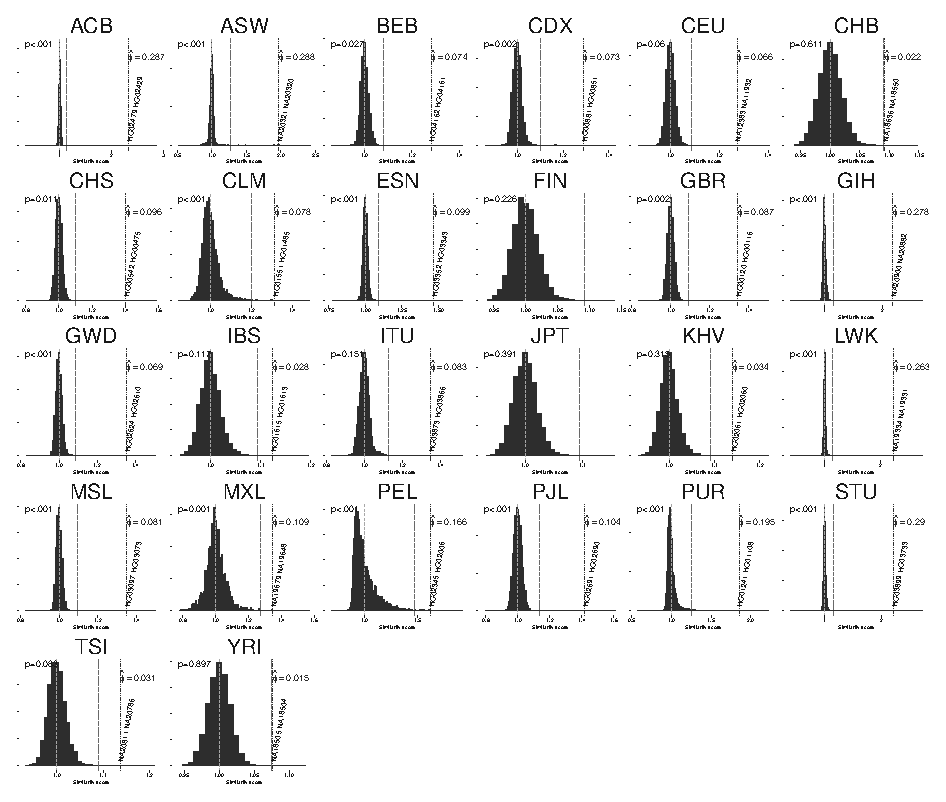
\includegraphics[]{./figures/figure1_bw.eps}
\caption[Distribution of similarity coefficients in the 1000 Genomes Project]{Distribution of similarity coefficients for each of the 26 populations
in the 1000 Genomes Project. Homogeneous populations lacking cryptic
relatedness should be expected to exhibit distributions centered around
1 with no outliers. The red dotted vertical line on each plot indicates
the family-wise$\alpha=.01$ level cutoff for ${n \choose 2}$ comparisons.
The most significant related pair is labeled for each population with
the estimated kinship for that pairing indicated in blue. The p-value
for the KS test for homogeneity is reported for each population. Many
of the population groups do demonstrate the null behavior (e.g. JPT,
KHV, FIN), however, a number of populations show the presence of extreme
outliers (e.g. STU, PUR) or systematic right skew (e.g. MXL, PEL)}
\label{fig: All s plots}
\end{figure*}

\begin{figure}
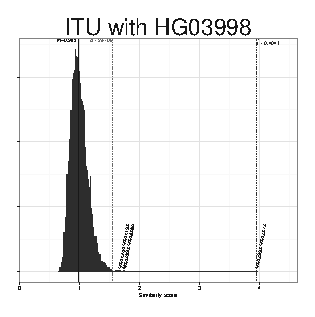
\includegraphics[width=1\columnwidth]{./figures/figure2_bw.eps}\caption[$s$ statistics for population Indian
Telugu from the UK with HG03998]{Distribution of all pairwise $s$ statistics for population Indian
Telugu from the UK (ITU) with individual HG03998 included. HG03998
is now believed to be related to HG03873, despite being labeled in
the Sri Lankan Tamil from the UK (STU) population. The family-wise
$\alpha=.01$ cutoff is indicated by the dotted red vertical line
and the $s$ statistic for HG03998 and HG03873 is seen as an extreme
outlier at 3.97.}
\label{fig: ITU with HG03998}
\end{figure}

\begin{figure*}
\includegraphics[width=1\columnwidth]{./figures/figure3.eps}
\caption[Significance of population heterogeneity in 26 populations
of the TGP]{\textbf{Significance of population heterogeneity in 26 populations
of the TGP}. Detection of population structure was found at $p<.01$
in 15 of the 26 populations using the full dataset (A). Upon removal
of suspected related individuals, four populations (CLM, PEL, PUR
and GIH) violated homogeneity in the relatedness-removed populations
(B).}
\label{fig: Structure pvals}
\end{figure*}


\subsection{Population differentiation in 1000 Genomes Project}

There are many methods for detecting population structure. Most commonly,
Principal Components Analysis (\citealp{price2006principal,price2010new})
is used, identifying the vectors of largest variation which
ideally corresponds to the population structure. Commonly, this procedure first
involves the computation of a genetic similarity matrix (GSM) via
the correlation between all samples, which is followed by
an eigendecomposition of that matrix. There are a number of limitations
to this straightforward approach, one of which is that the calculation
of a variance-covariance matrix equally weights the impact of all
loci, failing to fully utilize the fact that each variant's allele frequency
is informative of the value of each variant. Recently, the use of
the Jaccard Index has been used to estimate genetic similarity (\citealp{prokopenko2016utilizing}).
This approach provides a higher resolution picture of the genetic
landscape by exploiting the co-occurrence of rare-variants in sequencing
data. STEGO directly utilizes this the differential value of alleles
based on minor allele frequency by weighting variants by how unlikely
such a co-occurrence would have been in a homogeneous population. 

We evaluated the effectiveness of our similarity measure to differentiate
populations in the TGP in both global and localized contexts. For
the global scenario we used data from all 26 populations in a single
analysis. In the localized scenarios, we ran 57 separate analyses
corresponding to all possible pairs of populations within each of
the five superpopulations. In each analysis, STEGO and covariance (PCA) were used to compute
the GSMs containing all pairwise similarity scores. An eigendecomposition
of each GSM was performed and each individual in the study was plotted
against the top two eigenvectors for each method. 

In comparing our results with those of PCA on the global scale, we achieve highly similar
results depicting the two dimensional linear migrations
of ancient human history. This is notable because despite a focus on separating recently
related populations, STEGO remains effective at partitioning samples of
more distant common ancestry as well (Figure \ref{fig: heatmaps}). 

\begin{figure}
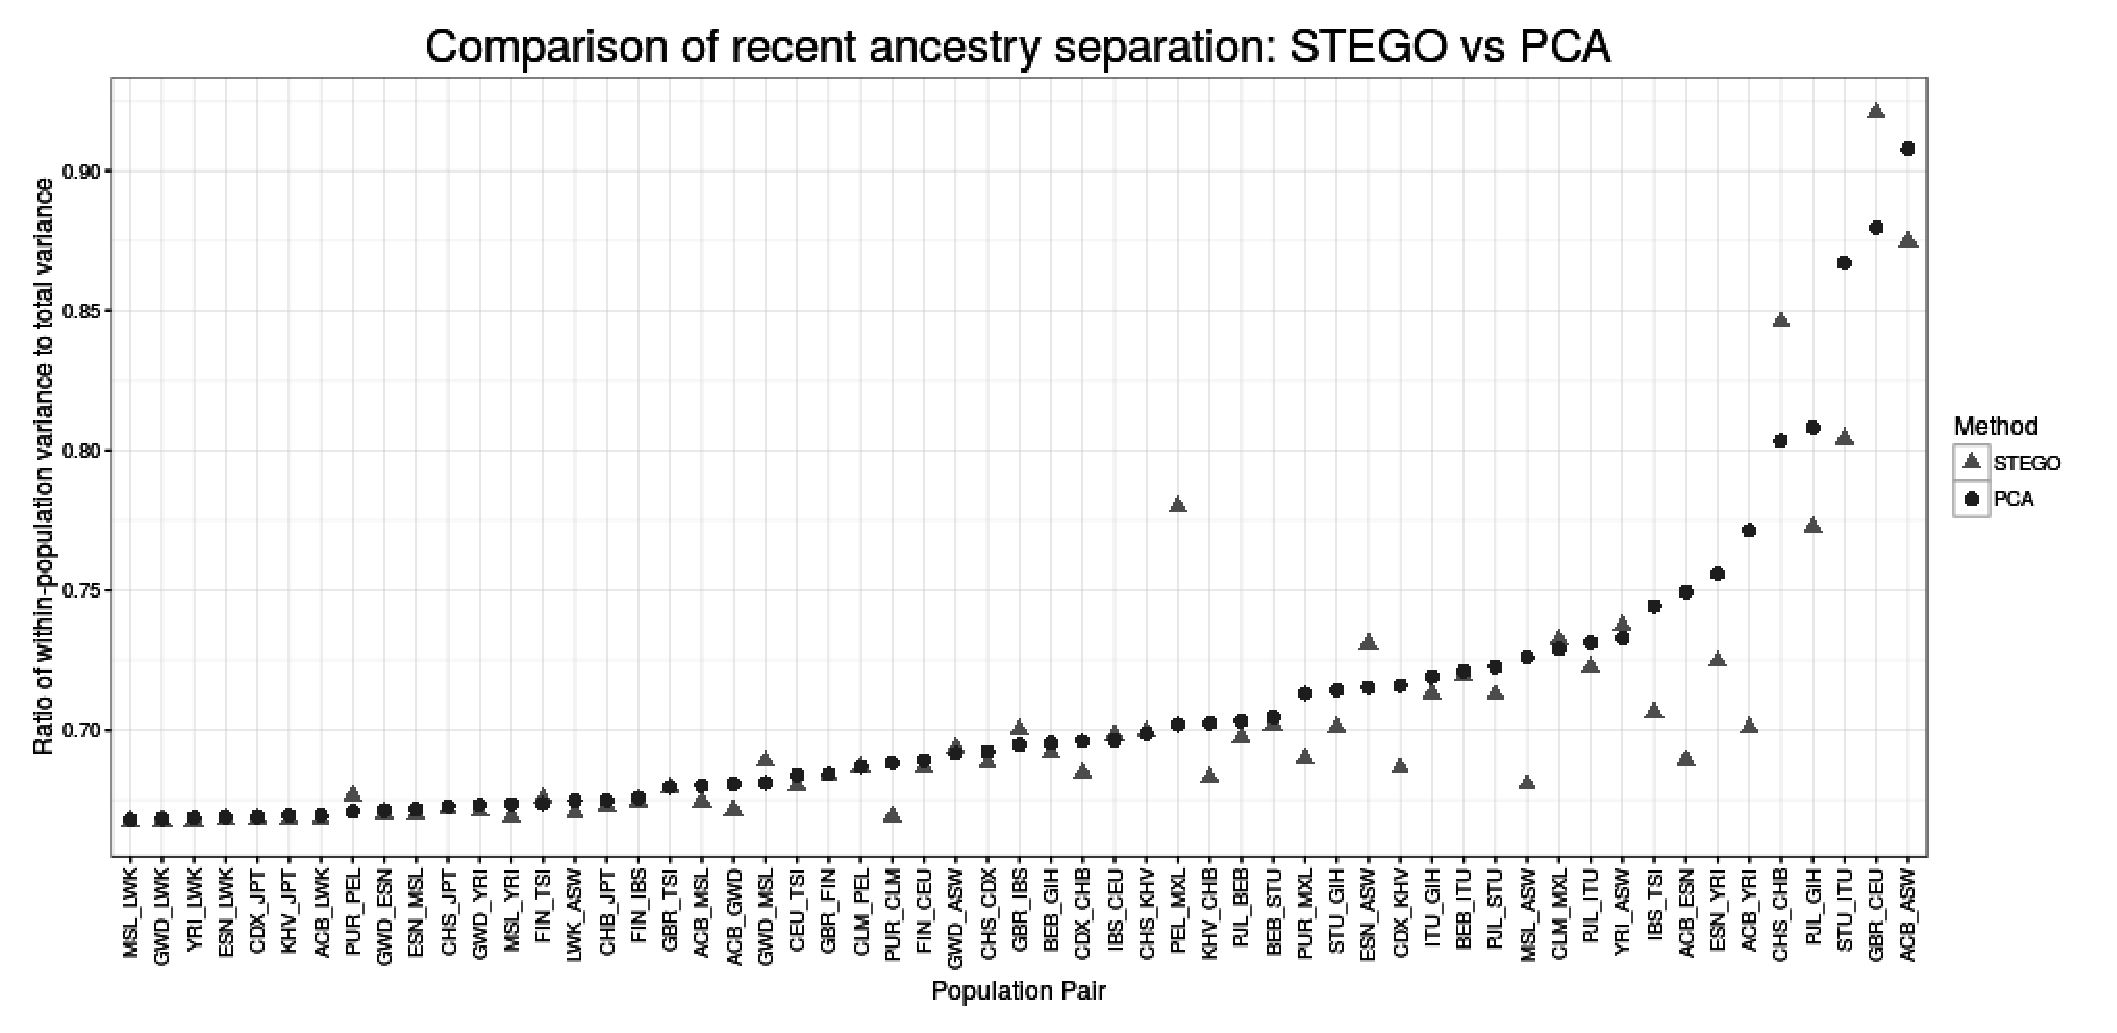
\includegraphics[width=1\columnwidth]{./figures/figure4_bw.eps}
\caption[Eigendecomposition separation using STEGO matrix and covariance]{The eigendecomposition of the STEGO matrix separates individuals of populations belonging to the same continent with greater efficiency than PCA. In 43 of 57 possible within-continent population pairs, STEGO had superior separation of populations. Separation was measured as the ratio of within population variance to total variance along the first 3 eigenvectors for STEGO and PCA. }
\label{fig: pairwise_variances}
\end{figure}

Despite no loss of performance on the global scale, STEGO outperforms standard PCA when the task involves classifying
individuals of recent ancestry. Focusing only on populations belonging
to the same continental superpopulation, every possible pair of populations were
merged following the removal of suspected related pairs. This yielded 57 sets of unrelated samples in which a subtle binary population stratification existed. STEGO and
standard PCA were then run on each merged dataset and the two methods
were compared by computing the ratio of mean within-population variance
to total variance across the first three principal components. 

The results show that STEGO outperforms PCA by this measure in 41
of the 57 possible comparisons (binomial test $p<.001$) (Figure \ref{fig: pairwise_variances}). We chose a pair of closely related populations from the
1000 Genomes Project in order to illustrate this performance. The
populations Sri Lankan Tamil (STU) and Indian Telugu (ITU) have relatively
small geographical separation and recent common ancestry relative
to other populations in the TGP. We demonstrate the clearer separation in comparing our method with that of standard Principal Components Analysis (Figure \ref{fig: ITUvsSTU}).  We additionally explored a case in which the ratio of mean within-population variance
to total variance was greater for STEGO compared to PCA, a group containing Utah Residents with Northern and Western Ancestry (CEU) and British in England and Scotland (GBR).  Despite a clear trend of superior performance with STEGO, CEU-GBR is a notable exception. Closer inspection reveals that the first eigenvector from STEGO clearly isolates 11 samples exclusively from the GBR population. To our knowledge, these individuals have not previously been identified as a distinct subset of the CEU population. It is not readily apparent what features of the data are being captured here or the relative value of those features (this may be a result of population structure, relatedness, batch effect, etc.). But it is notable that all 11 samples came from the same population in the TGP. It is reasonable to infer that this subset of samples contains a disproportionate number of co-occurrences of low frequency variants, which were not detected by PCA (Figure \ref{fig:CEU_GBR_comparison}).

The reasoning behind the superior performance in fine scale population
stratification is due to the focus on rarer alleles. Rare alleles
tend to be less stable over generations and become fixed at 0\% with
high probability. Therefore, rare alleles that are observed are more
likely to have arisen recently (see subsection "Ancestry informativeness by allele frequency"). It stands to reason that these alleles
would therefore be the most informative of recently related populations.
By appropriately recognizing the increased information contained in
the co-occurrences of less frequent alleles, we achieve superior separation
of recently related populations.

\begin{figure}
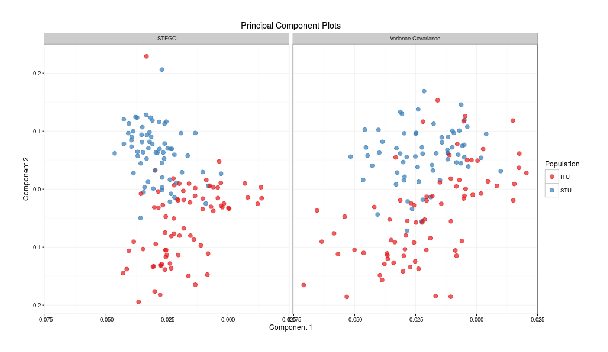
\includegraphics[width=1\columnwidth]{./figures/figure5.eps}
\caption[Separation of ITU vs STU comparison of methods]{\textbf{Example: ITU vs STU}. Two populations of Southern Asian origin,
Indian Telugu from the UK (ITU) and Sri Lankan Tamil from the UK (STU).
A genetic similarity matrix was computed using STEGO and standard
correlation on the same set of variants. An eigendecomposition of each matrix was then performed. These
plots show the set of unrelated individuals projected on to the first
two eigenvectors. We see clearer clustering by population (colored)
in our method (Left) compared to standard PCA (right). This performance
boost is attributed to the value added by preferentially considering
genetic agreement in less frequent alleles.}
\label{fig: ITUvsSTU}
\end{figure}


\section{Discussion}

The ability to identify genetic outliers has well-established utility
in genome-wide association studies. Many existing methods for identification
of genetic associations are predicated on the assumptions that population
homogeneity holds in the study. Checking for violations of these assumptions
typically involves a qualitative assessment without any specific concern
for effect size and power. STEGO provides an analytical approach for
quantitatively assessing homogeneity and a formal test for the identification
of cryptic relatedness and population stratification.  

Moreover, our approach involves the estimation of a GSM which, due to its preferential weighting towards rare variants, provides higher resolution for distinguishing populations which have recently diverged.  As sequencing costs have plummeted and our ability to measure rare variants has increased, there will be increased demand for tools which make use of the differential informativeness of variants according to frequency.  Recent work (\citealp{chen2013improved}) has already demonstrated the use of pre-calculated SNP weights to infer the ancestry of samples of unknown origin, and STEGO's GSM in combination with large scale sequencing projects, such as the TGP, promises to further improve the resolution of this approach.

Several limitations exist with our approach. First, the method assumes
that the variants are independent. We satisfy this assumption by performing
LD sampling, but in doing so limit the number of informative markers
to less than 100k, potentially omitting much of our data and reducing
our power to detect heterogeneity. The choice of LD
sampling method will necessarily impact the performance of the method, but due to the nature of STEGO focusing on rare variants as opposed to SNPs, the impact of LD will be limited.
Additionally, with respect to the detection of population structure,
we cannot design a uniformly most powerful test for structure due
to the complex nature in which structure can exist.  Future work will include quantification of the specific gains achieved in controlling type I error and power in the context of rare variant association studies.  Higher resolution population structure is always preferred, though the exact gains achieved in GWAS remain to be quantified.

In spite of these limitations, STEGO provides a formal, interpretable
tool which is directly linked to the kinship coefficient. It provides
a formal statistical test for population substructure, identifying
study subjects which are related and subjects which are genetic outliers
in their assigned population. 


\section*{Acknowledgements}

This work was supported by the National Institutes of Health [Grant numbers 1P01HL105339, T32HL007427] and Cure Alzheimer. The computations in this paper were run on the Odyssey cluster supported by the FAS Division of Science, Research Computing Group at Harvard University.\vspace*{-12pt}


\begin{figure}
\textbf{Distribution of similarity statistic within population subgroups
from 1000 Genomes Project after removal of related individuals}

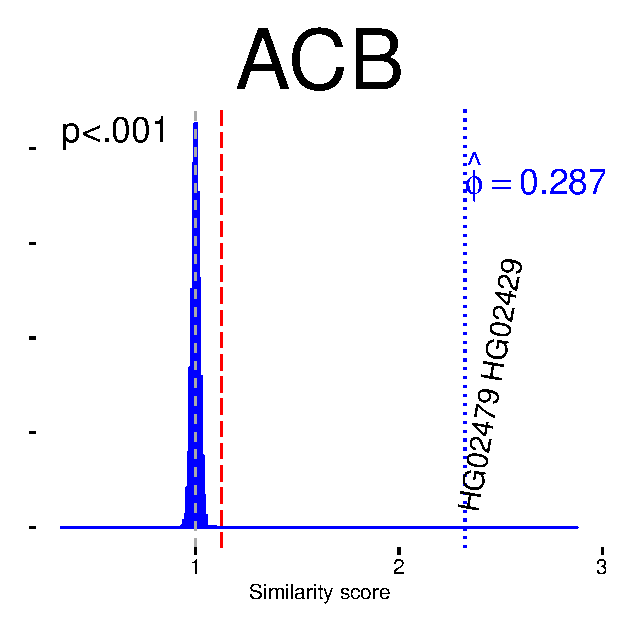
\includegraphics[width=0.12\paperwidth]{figures/PostFilter/ACBdiploid}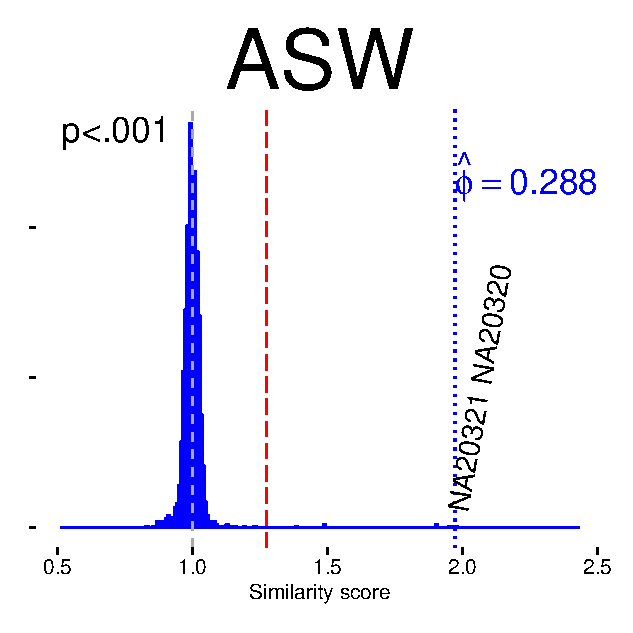
\includegraphics[width=0.12\paperwidth]{figures/PostFilter/ASWdiploid}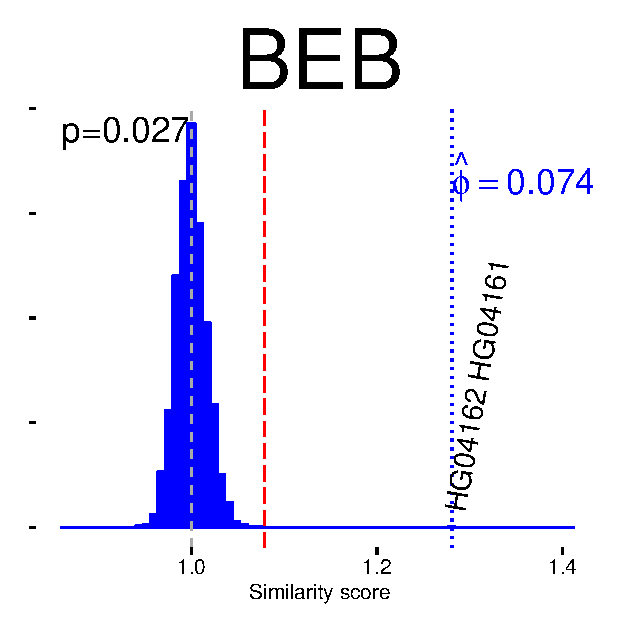
\includegraphics[width=0.12\paperwidth]{figures/PostFilter/BEBdiploid}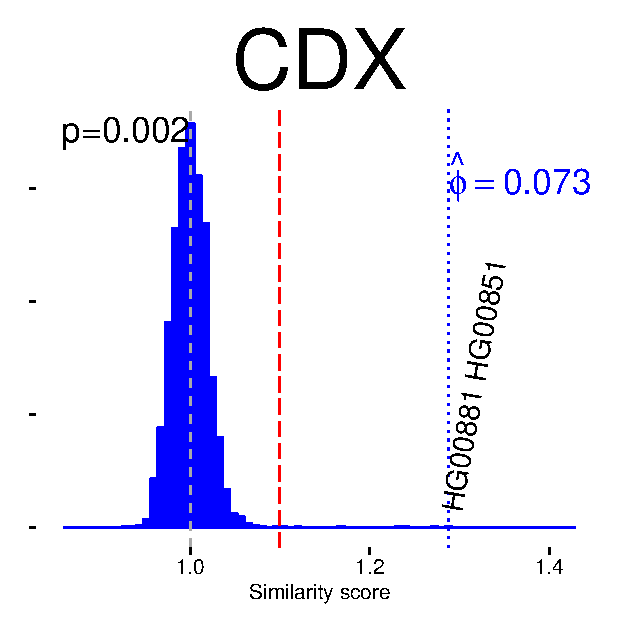
\includegraphics[width=0.12\paperwidth]{figures/PostFilter/CDXdiploid}\includegraphics[width=0.12\paperwidth]{figures/PostFilter/CEUdiploid}\includegraphics[width=0.12\paperwidth]{figures/PostFilter/CHBdiploid}

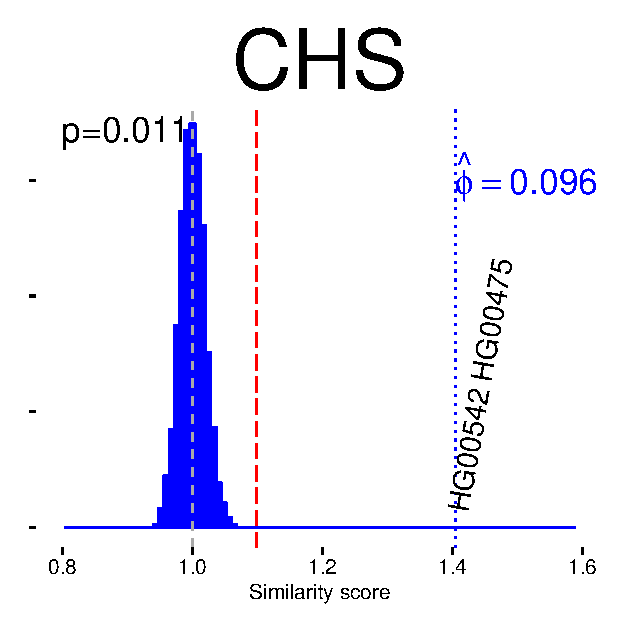
\includegraphics[width=0.12\paperwidth]{figures/PostFilter/CHSdiploid}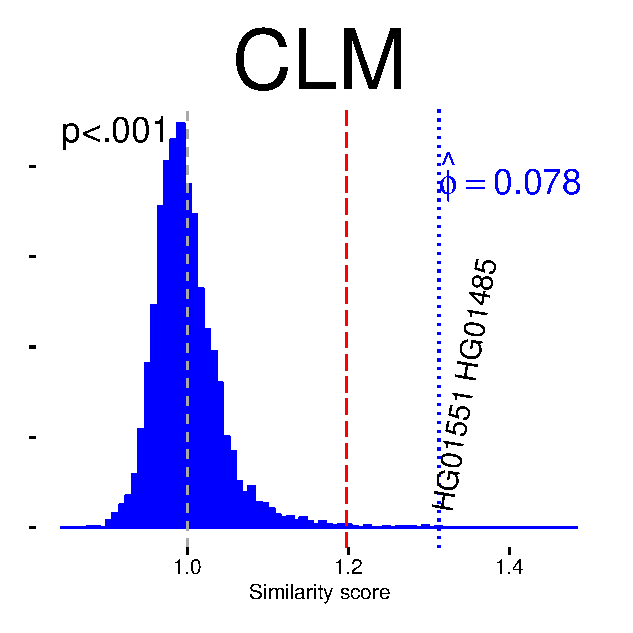
\includegraphics[width=0.12\paperwidth]{figures/PostFilter/CLMdiploid}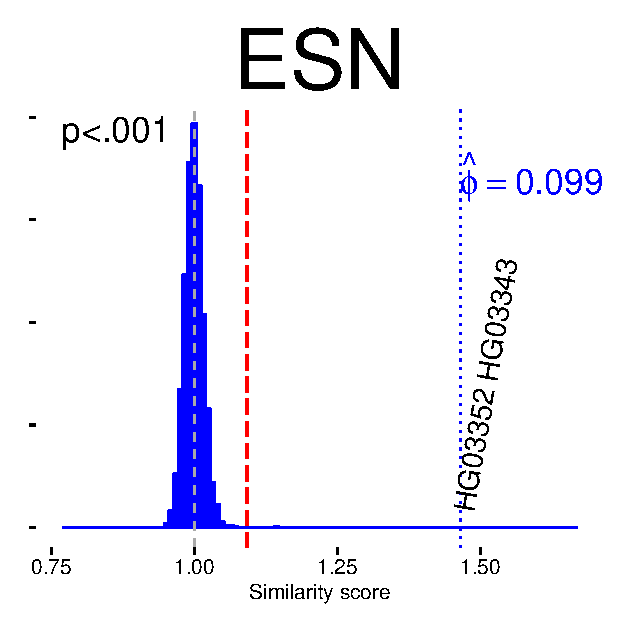
\includegraphics[width=0.12\paperwidth]{figures/PostFilter/ESNdiploid}\includegraphics[width=0.12\paperwidth]{figures/PostFilter/FINdiploid}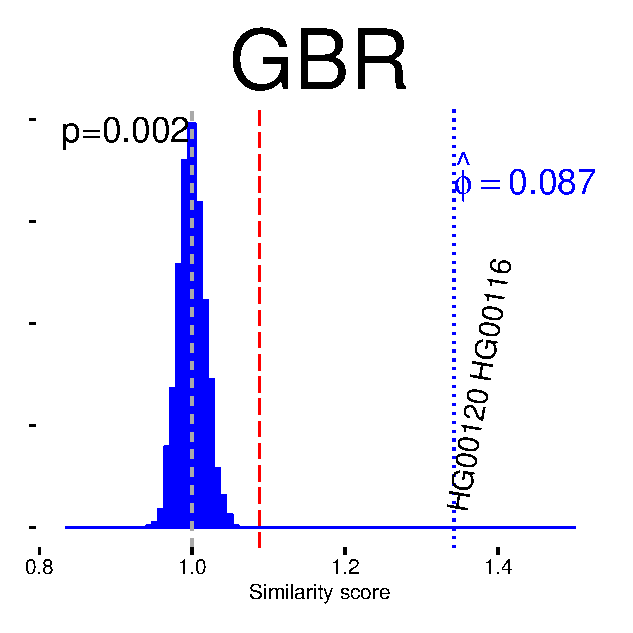
\includegraphics[width=0.12\paperwidth]{figures/PostFilter/GBRdiploid}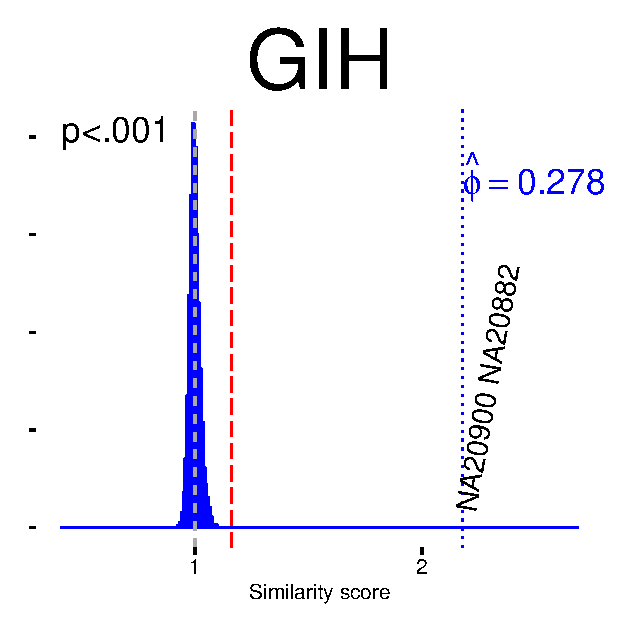
\includegraphics[width=0.12\paperwidth]{figures/PostFilter/GIHdiploid}

\includegraphics[width=0.12\paperwidth]{figures/PostFilter/GWDdiploid}\includegraphics[width=0.12\paperwidth]{figures/PostFilter/IBSdiploid}\includegraphics[width=0.12\paperwidth]{figures/PostFilter/ITUdiploid}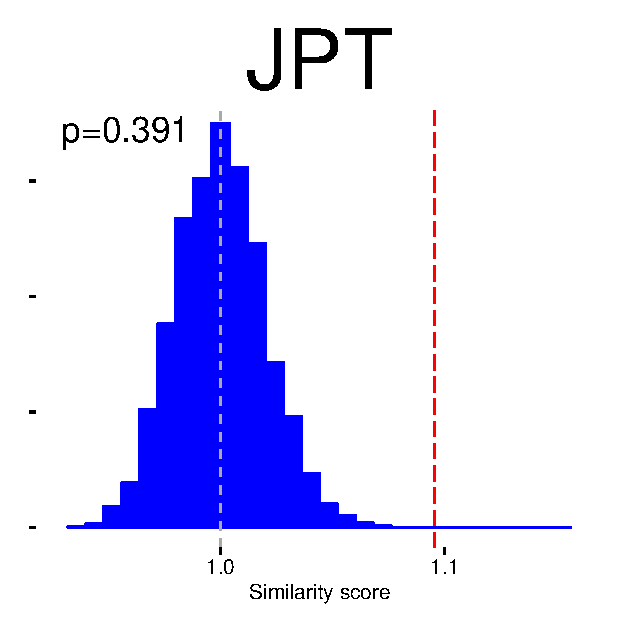
\includegraphics[width=0.12\paperwidth]{figures/PostFilter/JPTdiploid}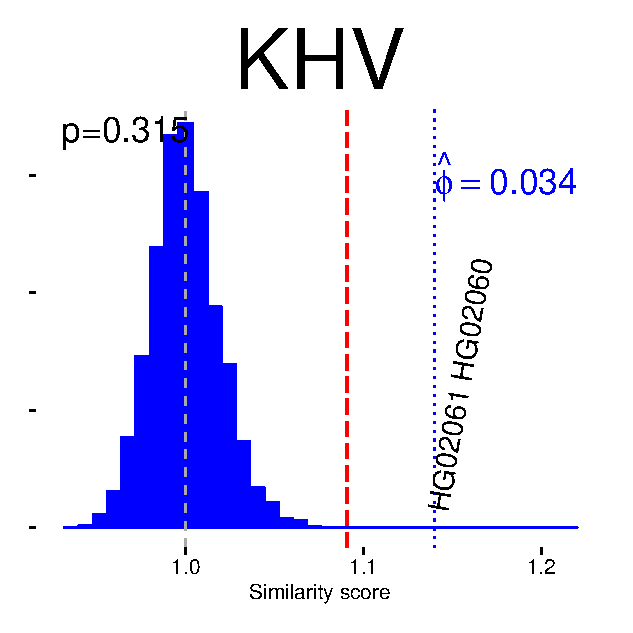
\includegraphics[width=0.12\paperwidth]{figures/PostFilter/KHVdiploid}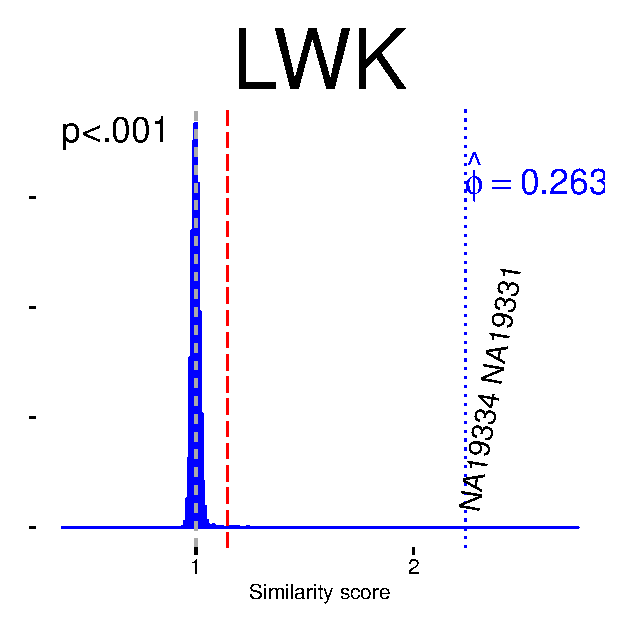
\includegraphics[width=0.12\paperwidth]{figures/PostFilter/LWKdiploid}

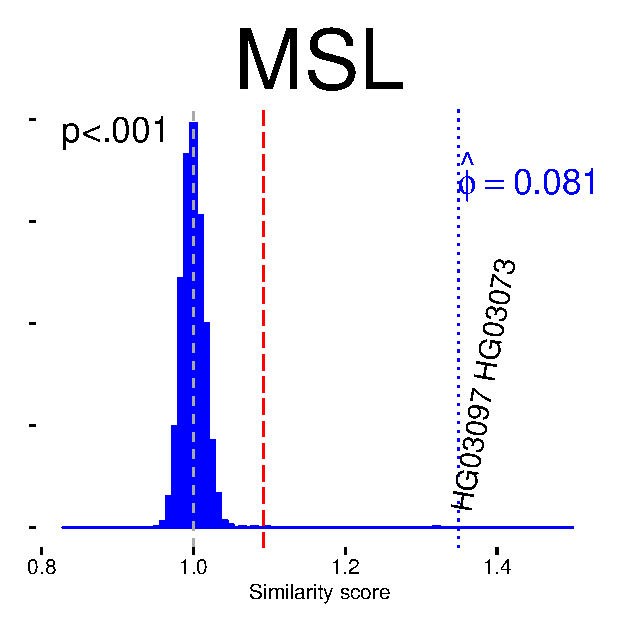
\includegraphics[width=0.12\paperwidth]{figures/PostFilter/MSLdiploid}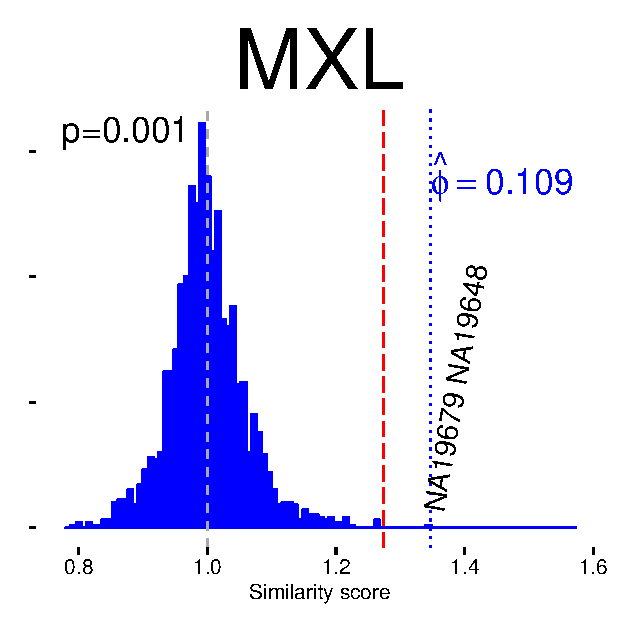
\includegraphics[width=0.12\paperwidth]{figures/PostFilter/MXLdiploid}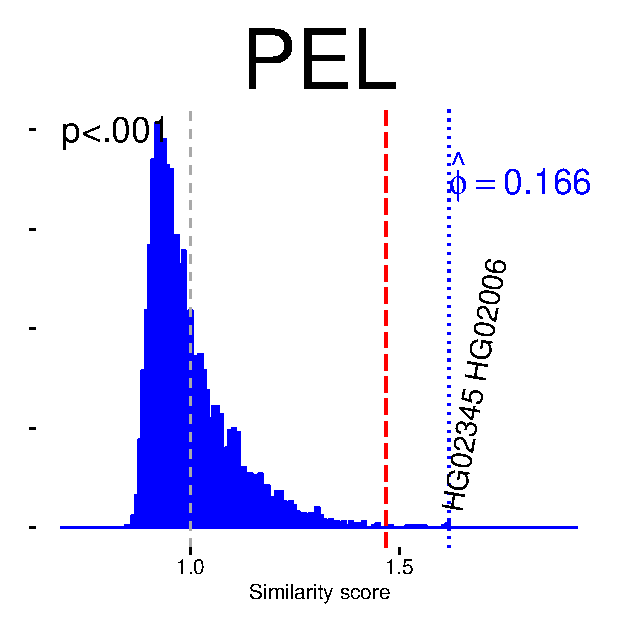
\includegraphics[width=0.12\paperwidth]{figures/PostFilter/PELdiploid}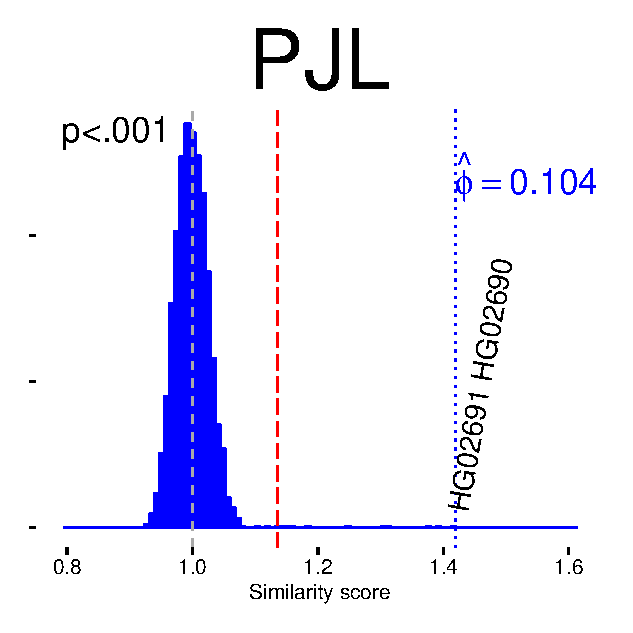
\includegraphics[width=0.12\paperwidth]{figures/PostFilter/PJLdiploid}\includegraphics[width=0.12\paperwidth]{figures/PostFilter/PURdiploid}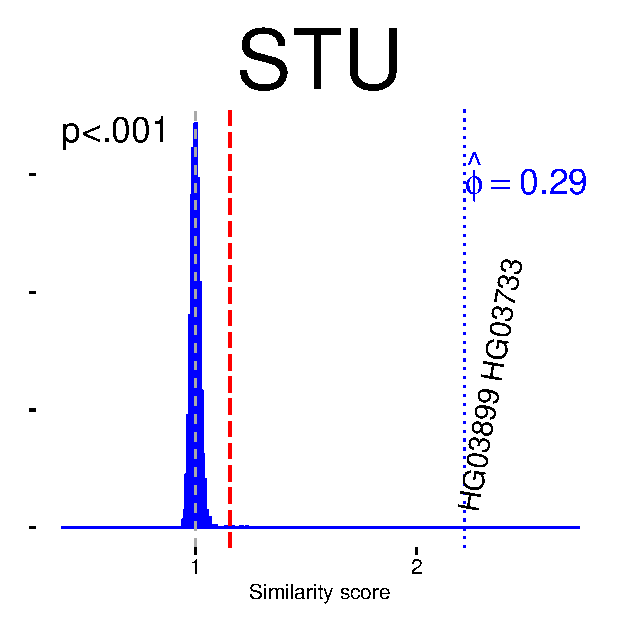
\includegraphics[width=0.12\paperwidth]{figures/PostFilter/STUdiploid}

\includegraphics[width=0.12\paperwidth]{figures/PostFilter/TSIdiploid}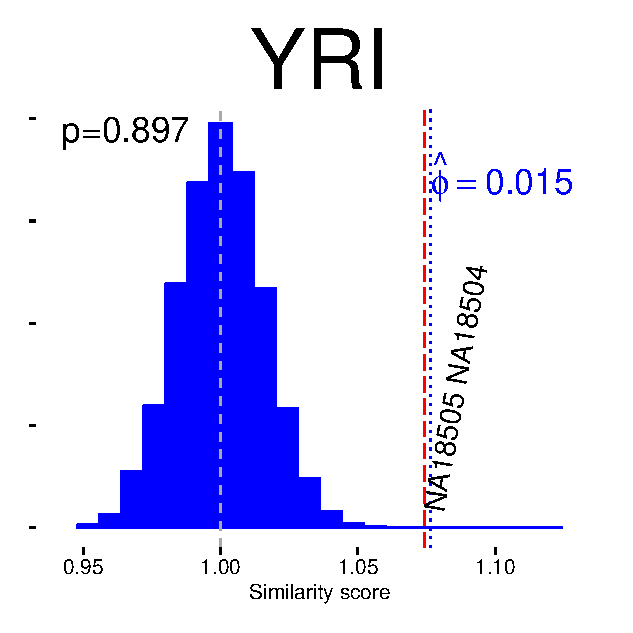
\includegraphics[width=0.12\paperwidth]{figures/PostFilter/YRIdiploid}\caption[Similarity coefficients for each population
in the 1000 Genomes Project]{Distribution of similarity coefficients for each of the 26 populations
in the 1000 Genomes Project after the removal of suspected related
individuals. Homogeneous populations lacking cryptic relatedness should
be expected to exhibit distributions centered around 1 with no outliers.
A heterogeneous population is expected to exhibit a normal distribution
centered around 1. Non-normal distributions such as right-skewed (e.g.
PUR, PEL, CLM) or bimodal are indicative of population structure.
The red dotted vertical line on each plot indicates the family-wise$\alpha=.01$
level cutoff for ${n \choose 2}$ comparisons. The most significant
related pair is labeled for each population with the estimated kinship
for that pairing indicated in blue. The p-value for the KS test for
homogeneity is reported for each population. Outliers in the absence
of non-normally distributed statistics are an indication of relatedness
among pairs of individuals.}
\label{All s plots-1}
\end{figure}

\begin{figure}
\textbf{A}\includegraphics[width=0.75\columnwidth]{figures/GSM_trim}

\textbf{B}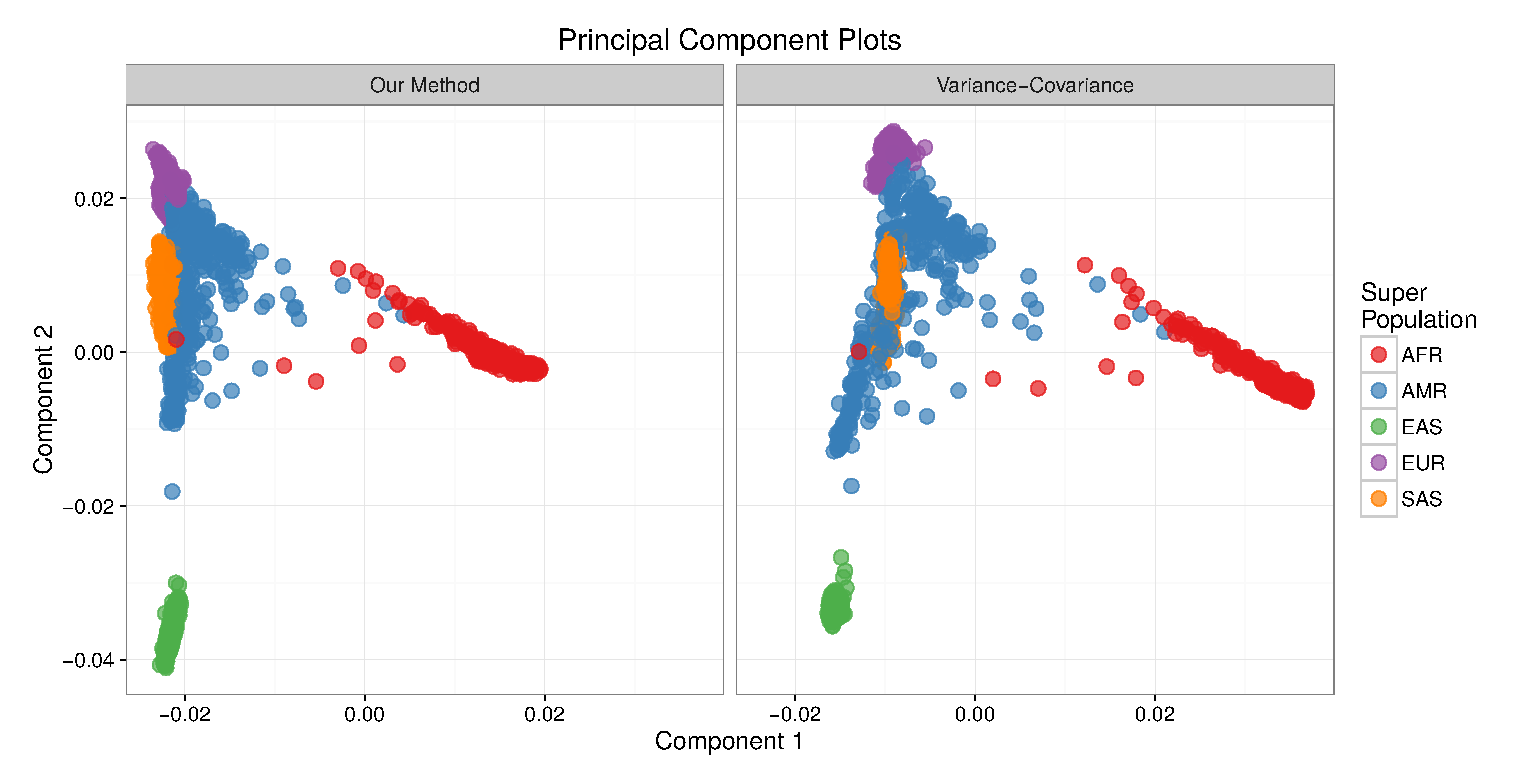
\includegraphics[width=0.8\columnwidth]{figures/PCA_all}\caption[Population structure within populations of 1000 Genomes Project.]{Population structure in 2504 samples from 1000 Genomes Project. (\textbf{A})
Heatmap of the GSM generated by STEGO using 80,000 LD-sampled variants.
The vertical colorbar indicates membership in one of the five superpopulations,
while the horizontal colorbar indicates membership in one of the 26
populations. (\textbf{B}) Projecting each individual onto the top
two eigenvectors resulted in a similar 2-dimensional distribution
of global ancestry. Both STEGO and PCA show similar projections which
elucidate the migratory patterns of early humans.}
\label{fig: heatmaps}
\end{figure}
\begin{figure}
\includegraphics[width=1\columnwidth]{./figures/PCA_CEU_GBR}\caption[Similarity coefficients for populations GBR
and CEU]{Despite a clear trend of superior performance with STEGO, notable
exceptions occur. For example, by this measure, the populations GBR
and CEU were more clearly divided by PCA (Right) than by STEGO (Left).
Closer inspection revealed that the first eigenvector from STEGO isolates
11 samples exclusively from the GBR population. It is not readily
apparent what features of the data are being captured here or the
relative value of those features (this may be a result of population
structure, relatedness, batch effect, etc.). But it is notable that
all 11 samples came from the same population in the 1000 Genomes Project.
It is reasonable to infer that this subset of samples is scientifically
relevant. It most likely contains a disproportionate number of co-occurences
of rare variants, which were not observed separately by PCA.}
\label{fig:CEU_GBR_comparison}
\end{figure}

\begin{figure}
 \resizebox{\columnwidth}{!}{%

\includegraphics{/home/dan/1000GP/supplemental_figure_wk}

}\caption[Distribution of weight factor]{The weight factor, $w_{k}$, is shown here as a function of the minor
allele count in an example of 100 individuals (200 alleles) for each
locus, $k$. $w_{k}$ is monotonically decreasing for minor allele
counts greater than $1$, lending greater power to lower frequency
variants.  Typically, there will be a minimum minor allele count such
that the largest values for $w_{k}$are never obtained in practice}
\end{figure}

\begin{figure}
\includegraphics[width=1\columnwidth]{/home/dan/1000GP/plots/YRIvsAll_continent_color_interval}\label{YRIvsX}\caption[Allele informativeness by minor frequency]{\textbf{Lower frequency alleles are more informative of ancestry.
}For the Yoruban population (YRI), this plot compares the average
unweighted Jaccard Index between individuals within group the to individuals
in all other populations of the 1000 Genomes Project. When filtering
by each minor allele frequency, we observe that low frequency alleles
create the strongest separation between populations. This trend holds
true for all but the lowest interval (0-0.4\% MAF), likely owing to
a tradeoff between rare variant informativeness and quality control
reliability.}
\label{fig:supp_fig5}
\end{figure}

\begin{figure}
\includegraphics[width=1\columnwidth]{/home/dan/1000GP/average_timing_comparison}\caption[Running time comparison of STEGO , \textbf{cor()} and \textbf{princomp()} in R]{\textbf{Average running time of STEGO is compared to the default implementations
of \textbf{cor()} and \textbf{princomp()} in R.} For each sample
size on the x-axis, 100,000 variants were randomly generated across
the samples. R functions for STEGO, correlation, and two implementations
of PCA (\textbf{prcomp }and \textbf{princomp}) were run 10 times on
each simulated dataset. Each of these methods has asymptotic computational
complexity of $\mathcal{O}(pN^{2})$, and we observe a consistent
speed improvement of approximately 3x for STEGO compared to \textbf{princomp()}.
This improvement scales linearly with increased number of variants,
which is most appealing for large whole genome sequencing studies
involving thousands of subjects and millions of variants.}
\label{comp_time}
\end{figure}

\begin{figure}
\includegraphics[width=1\columnwidth]{/home/dan/1000GP/simulated_PCP_plots}\caption[Simulated Principal Component plots for two methods for generating the genetic
similarity matrix]{Principal Component plots for two methods for generating the genetic
similarity matrix. On the left, the GSM is generated via STEGO and
on the right the GSM uses the normalized covariance matrix. The STEGO
method makes more efficient use of the more ancestry informative rare
variants, providing a higher resolution separation of our two closely
related populations. Across the first two components the ratio of
within-population variance to total variance for STEGO vs variance-covariance
is .81 and .99, respectively.}
\label{simulatedPCP}
\end{figure}

\begin{figure}
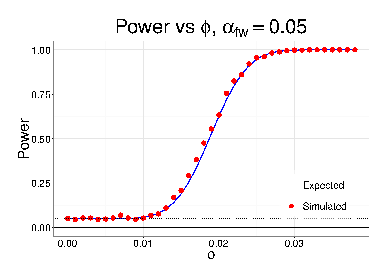
\includegraphics[width=1\columnwidth]{./figures/power_curve}\caption[Power curve for detection of related pair]{The probability of rejecting the null hypothesis given a simulated
set of 301 homogeneous individuals containing a single related pair
with coefficient of kinship, $\phi$. The simulated power curve aligns
with the analytically derived expectation demonstrating the clearly
defined power of the method.}
\label{power_curve}
\end{figure}

\begin{table}
\begin{tabular}{|c|c|c|c|}
\hline 
Population & Super Population & Structure & Cryptic Relatedness\tabularnewline
\hline 
\hline 
ACB & \multirow{7}{*}{AFR - African} & NO & NO\tabularnewline
\cline{1-1} \cline{3-4} 
ASW &  & NO & \textbf{YES}\tabularnewline
\cline{1-1} \cline{3-4} 
ESN &  & NO & NO\tabularnewline
\cline{1-1} \cline{3-4} 
GWD &  & NO & NO\tabularnewline
\cline{1-1} \cline{3-4} 
LWK &  & NO & NO\tabularnewline
\cline{1-1} \cline{3-4} 
MSL &  & NO & NO\tabularnewline
\cline{1-1} \cline{3-4} 
YRI &  & NO & YES\tabularnewline
\hline 
CLM & \multirow{4}{*}{AMR - Ad Mixed American} & \textbf{YES} & \textbf{YES}\tabularnewline
\cline{1-1} \cline{3-4} 
MXL &  & NO & NO\tabularnewline
\cline{1-1} \cline{3-4} 
PEL &  & \textbf{YES} & \textbf{YES}\tabularnewline
\cline{1-1} \cline{3-4} 
PUR &  & \textbf{YES} & \textbf{YES}\tabularnewline
\hline 
CDX & \multirow{5}{*}{EAS - East Asian} & NO & NO\tabularnewline
\cline{1-1} \cline{3-4} 
CHB &  & NO & NO\tabularnewline
\cline{1-1} \cline{3-4} 
CHS &  & NO & NO\tabularnewline
\cline{1-1} \cline{3-4} 
JPT &  & NO & NO\tabularnewline
\cline{1-1} \cline{3-4} 
KHV &  & NO & NO\tabularnewline
\hline 
CEU & \multirow{5}{*}{EUR - European} & NO & NO\tabularnewline
\cline{1-1} \cline{3-4} 
FIN &  & NO & NO\tabularnewline
\cline{1-1} \cline{3-4} 
GBR &  & NO & NO\tabularnewline
\cline{1-1} \cline{3-4} 
IBS &  & NO & NO\tabularnewline
\cline{1-1} \cline{3-4} 
TSI &  & NO & NO\tabularnewline
\hline 
BEB & \multirow{5}{*}{SAS - South Asian} & NO & NO\tabularnewline
\cline{1-1} \cline{3-4} 
GIH &  & \textbf{YES} & NO\tabularnewline
\cline{1-1} \cline{3-4} 
ITU &  & NO & NO\tabularnewline
\cline{1-1} \cline{3-4} 
PJL &  & NO & NO\tabularnewline
\cline{1-1} \cline{3-4} 
STU &  & NO & NO\tabularnewline
\hline 
\end{tabular}\caption[Presence of population structure and cryptic relatedness detected
in each of the 26 populations in the 1000 Genomes Project]{\textbf{Presence of population structure and cryptic relatedness detected
in each of the 26 populations in the 1000 Genomes Project.} STEGO
was run separately on each population group following the removal
of suspected related individuals. Population structure was defined
as a significant $\left(p<.01\right)$ Kolmogorov-Smirnov statistic
comparing the observed test statistic distribution to that expected
under the assumption of homogeneity. Cryptic relatedness was defined
as those populations containing at least one pair of individuals with
estimated kinship $\hat{\phi}>\frac{1}{32}$ and statistically significant
$\left(p<.01\right)$ kinship after multiple testing correction. }

\label{population_table}
\end{table}